\chapter{Tsoureki}
\label{ch:tsoureki}
\index{dessert}
\index{bread}
\index{mahleb}
\index{Easter}

\marginnote{
    \textbf{Makes ? round braids} \\
    Prep time: 6+ hours \\
    Cook time: 30-45 minutes \\
    \vspace*{\baselineskip}

    \textbf{Ingredients for dough} \\
    11 cups all purpose flour (Five Roses) \\
    1 1/2 cups sugar \\
    1 1/2 cups milk \\
    1 1/2 cups butter, melted and cooled \\
    8 eggs \\
    1 tsp mahleb \\
    1/2 tsp salt \\
    2 packets active yeast \\
    \vspace*{\baselineskip}

    \textbf{Ingredients to bake} \\
    Aluminium foil \\
    Colored Easter eggs \\
    2 eggs, for egg wash \\
    Slivered almonds
}

\textit{Easter bread}

Family member: Grandma Eleni

\newthought{Easter} is not Easter without \textgreek{τσουρέκι}! I can just think of the delicious smell as they're baking in the oven. If you would like to add a red Easter Egg, you can do so while shaping and bake it in the oven. Grandma \textgreek{Ελένη} would crumple a piece of foil and place it in the center of the circle to hold the shape while it bakes. Once cooled, she would remove the foil and replace it with a Easter Egg.

\begin{enumerate}
    \item  In a small bowl, put the yeast with a little bit of sugar and warm water. Mix and leave it for half an hour.
    \item  After half an hour, mix all the ingredients for the dough in a large bowl and leave it uncovered for 1 hour.
    \item  Once 1 hour has passed, shape in braids and let them rise uncovered for 6 hours.
    \item  Shape pieces of foil into small cylinders and place in the middle of each bun, where the painted eggs will go. Brush with egg wash and decorated with slivered almonds.
    \item  Bake at 350-400\degree F until the tops have a golden color and tsourekia are baked.
    \item  Let cool for a few hours. Remove the foil and replace with colored Easter eggs.
\end{enumerate}

\begin{figure}
  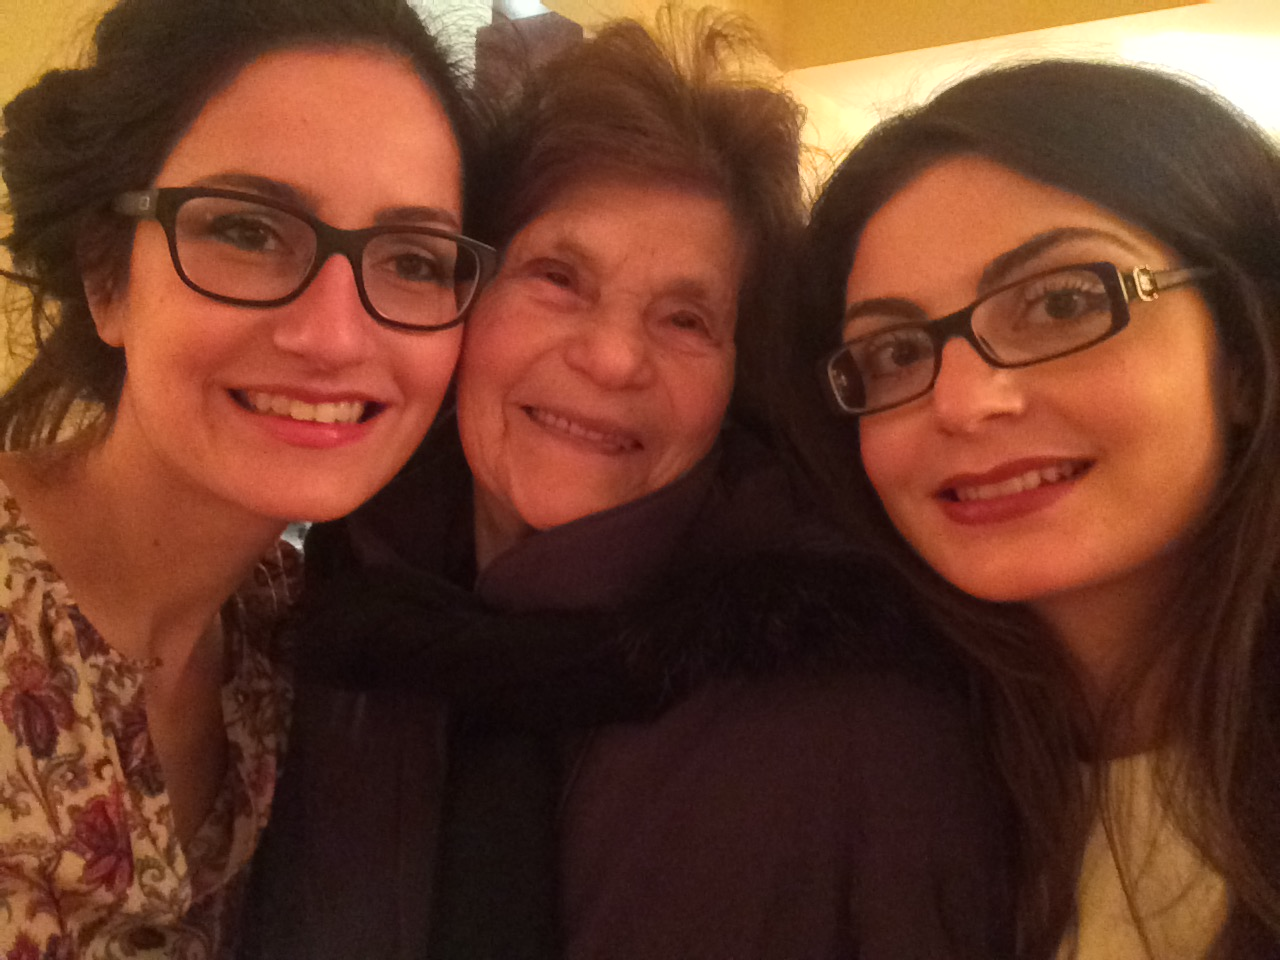
\includegraphics[width=60mm]{monanteras/images/Grandma eleni.JPG}
\end{figure}
